%%%%%%%%%%%%%%%%%%%%%%%%%%%%%%%%%%%%%%%%%
% Short Sectioned Assignment
% L	aTeX Template
% Version 1.0 (5/5/12)
%
% This template has been downloaded from:
% http://www.LaTeXTemplates.com
%
% Original author:
% Frits Wenneker (http://www.howtotex.com)
%
% License:
% CC BY-NC-SA 3.0 (http://creativecommons.org/licenses/by-nc-sa/3.0/)
%
%%%%%%%%%%%%%%%%%%%%%%%%%%%%%%%%%%%%%%%%%

%----------------------------------------------------------------------------------------
%	PACKAGES AND OTHER DOCUMENT CONFIGURATIONS
%----------------------------------------------------------------------------------------

\documentclass[paper=a4, fontsize=11pt]{scrartcl} % A4 paper and 11pt font size
%\documentclass{article}
\usepackage{algorithm}
\usepackage{algpseudocode}
\usepackage{pifont}
\usepackage{listings}
\usepackage{multirow}
\usepackage{hyperref}
\usepackage[T1]{fontenc} % Use 8-bit encoding that has 256 glyphs
\usepackage{graphicx} % Required for including images
%\usepackage{fourier} % Use the Adobe Utopia font for the document - comment this line to return to the LaTeX default
\usepackage[english]{babel} % English language/hyphenation
\usepackage{amsmath,amsfonts,amsthm} % Math packages

\usepackage{setspace}
\doublespacing

\usepackage[margin=1in]{geometry}

\usepackage{indentfirst}

\usepackage{lipsum} % Used for inserting dummy 'Lorem ipsum' text into the template

\usepackage{sectsty} % Allows customizing section commands
\allsectionsfont{\centering \normalfont\scshape} % Make all sections centered, the default font and small caps

\usepackage{fancyhdr} % Custom headers and footers
\pagestyle{fancyplain} % Makes all pages in the document conform to the custom headers and footers
\fancyhead{} % No page header - if you want one, create it in the same way as the footers below
\fancyfoot[L]{} % Empty left footer
\fancyfoot[C]{} % Empty center footer
\fancyfoot[R]{\thepage} % Page numbering for right footer
\renewcommand{\headrulewidth}{0pt} % Remove header underlines
\renewcommand{\footrulewidth}{0pt} % Remove footer underlines
\setlength{\headheight}{13.6pt} % Customize the height of the header

\numberwithin{equation}{section} % Number equations within sections (i.e. 1.1, 1.2, 2.1, 2.2 instead of 1, 2, 3, 4)
\numberwithin{figure}{section} % Number figures within sections (i.e. 1.1, 1.2, 2.1, 2.2 instead of 1, 2, 3, 4)
\numberwithin{table}{section} % Number tables within sections (i.e. 1.1, 1.2, 2.1, 2.2 instead of 1, 2, 3, 4)

\setlength{\parindent}{1cm} % Removes all indentation from paragraphs - comment this line for an assignment with lots of text

%----------------------------------------------------------------------------------------
%	TITLE SECTION
%----------------------------------------------------------------------------------------

%\newcommand{\horrule}[1]{\rule{\linewidth}{#1}} % Create horizontal rule command with 1 argument of height

%\title{	
%\normalfont \normalsize 
%\textsc{Wayne State University, CS} \\ [25pt] % Your university, school and/or department name(s)
%\horrule{0.5pt} \\[0.4cm] % Thin top horizontal rule
%\huge Face Verification Problem on the Large Scale Datasets \\ % The assignment title
%\horrule{2pt} \\[0.5cm] % Thick bottom horizontal rule
%}

%\author{PhD student: Artem Komarichev} % Your name

%\textsc{Advisor: Prof. Xuewen Chen} \\ [25pt]

%\date{\normalsize\today} % Today's date or a custom date

\begin{document}

\begin{titlepage}
    \begin{center}
        \vspace*{1cm}
        \LARGE
        Literature Survey \\
        \vspace{0.5cm}
        \Huge
        \textbf{Face Verification Problem on \\ the Large Scale Datasets}
        
        \vspace{0.5cm}
        \LARGE
        %Thesis Subtitle
        
        \vspace{5.5cm}
        
        Ph.D. candidate: \textbf{Artem Komarichev}
        
        Research advisor: \textbf{Prof. Xue-wen Chen}
        
        \vfill
        
        
        \vspace{0.8cm}
        
        
\includegraphics[scale=0.15]{pictures/warrior_banded_logo.jpg}
        
        \Large
        Department of Computer Science\\
        Wayne State University\\
        USA\\
        
    \end{center}
\end{titlepage}

%\maketitle % Print the title

%----------------------------------------------------------------------------------------
%	PROBLEM 1
%----------------------------------------------------------------------------------------

\newpage

\section{Introduction}

In the recent few years the interest in face recognition problems was increased significantly. One of the reasons behind this that now we have more powerful machines than couple decades ago which we can use to run more complex models. Moreover with the rapid grough in the development of convolutional netural networks (CNN) and deep architectures we could learn much better feature representations to make our predictions more accurate. But the interesting question which come to our mind: why did neural networks become so popular recently? And the answer is the following: Support Vector Machine (SVM), Linear Disciminant Analysis (LDA), and Principal Component Analysis (PCA) are showed bad scaling properties. On the other hand, deep neural networks (DNN) are more tolerate to the size of training dataset.\cite{taigman2014deepface}.


Plus, there are a plenty of potential areas where we can apply our models such as: biometrics, information security, law enforcement and surveillance, access control and many others \cite{zhao2003face}. \par
Face recognition can be divided into several directions:
\begin{itemize}
  \item face verification
  \item face identification
  \item face detection
  \item face clustering
\end{itemize}

The main goal of \textit{face verification} is to define whether two face images belong to the same person or not. \textit{Face detection} is basically defining are there faces in the image, and if it is true, just return their locations in this digital image \cite{yang2002detecting}. The goal of \textit{face identification} is to assign each image to appropriate class in a dabase \cite{seo2011face}. \textit{Face clustering} defines common people among all available face images in the database. I want to concentrate only on face verification problem in this literature survey. \par

What does make face recognition problem hard to be solved? Some: illumination, rotation, different poses, occlusion \cite{ekenel2009facial}, facial expressions and so on. One of the datasets which reflects these difficulties is PIE (pose, illumination, and expression) dataset \cite{sim2002cmu}. The examples of image pairs you can see in Fig. 1 (I will add image next time). And it was considered to be very difficult to solve until the guys from Google proposed their solution \cite{schroff2015facenet} and solved it.

The other issue which I would like to consider here is using of large-scale datasets in solving problem. In order to effectively run any face verfification model on huge dataset we most likely need to parallelize our solution. There is two possible ways to make this: model parallelization and data parallelization \cite{dean2012large}. I will cover them in more details later and show some state-of-the-art applications. \par

%Alongside with the development of deep conovolutional networks, the researchers %started to apply deep architectures in their models to solve face verification %problem. LDA, SVM was also applied (I need to find papers).\par 

I will also descibe two widely used datasets for evaluation: Labeled Faces in the Wild (LFW) and Youtube Faces DB (YTF).

\section{DeepFace}

Facebook presented their own DeepFace model \cite{taigman2014deepface} to solve face verification problem. In their paper, they are considering face images in unconstrained settings. Based on that, they proposed new 3D alignment process, and their own DNN architecture, which has nine layers, to learn good feature representations. Also they collected their own huge dataset with 4 million face images which belong to 4K unique identities. This dataset was used to train their DeepFace model.

\subsection{Face alignment}

Alignment is still considered to be difficult problem to solve especially in the unconstrained environment. In the recent few years 3D modeling was used extensively \cite{hassner2013viewing}. In this paper \cite{schroff2015facenet}, authors applied 3D modeling too to extract frontal faces. Simple steps is presented in the image below.\par

\begin{center}
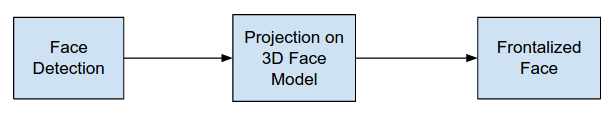
\includegraphics[scale=0.5]{pictures/front.png}
\par\large\textit{Figure ?.?: Frontalization steps.}
\end{center}

Frontalization. The first step is to detect face, they used 6 fiducial points to do this. Two points for eyes, one for the tip of nose, and three others to locate mouth. After that detected face was cropped. That is the final step in Face Detection process, see Figure ?.?. After that they added 67 more fiducial points as anchors and projected them on the 3D face model. Their 3D model was got by taking an average among all available 3D models in the USF Human-ID database. All these fiducial points was extracted applying Support Vector Regressor (SVR) algorithm. And the final step was to wrap 2D image to get frontal face of the original face image. 

\subsection{DeepFace architecture}

The main reason behind using feature representations learned through DNN instead of using handcrafted engineered features because they shows better prediction accuracy.  The more data available, the better features could be extracted using deep architectures. \par
The big picture of DeepFace model is represented below. \par

\begin{center}
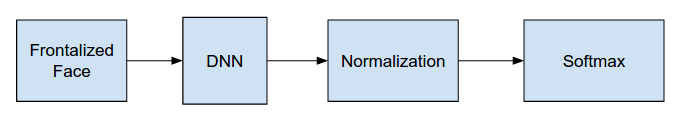
\includegraphics[scale=0.5]{pictures/deepface.png}
\par\large\textit{Figure ?.?: DeepFace architecture.}
\end{center}

Input signal to the DNN is a 3D-aligned faces in RGB. The size of the input image is $152 \times 152$ pixels. The process of getting 3D-aligned face images was described in the previous section.\par

Speaking of DNN architecture, it has two convolutional layers (C1$@11\times11\times32$ and C3$@9\times9\times16$), one max-pooling layer (M2:$3\times3, stride=2$), three locally connected layers (L4$@9\times9\times16$, L5$@7\times7\times16$, and L6$@5\times5\times16$) and final two fully connected layers (F7:$4096d$ and F8:$4030d$). The key difference between convolutional layer and locally connected (LC) one that there is no weights sharing across the whole image. Each patch in LC layer has his own filter. In contrast to LC layers, convolutional layers has one filter for every patch extracted from image. Having more parameters to train in the LC layers doesn't lead to an increase in computations. The only reason why they used this type of layers because they have pretty huge training dataset which made it possible to train them. The number of parameters was close to 120M, where 95$\%$ was from LC and FC layers. The last FC layer represents softmax classifier, where the number of classes is equal to 4030 unique identities in the training dataset. \par

As loss function was chosen cross-entropy loss, becuase the goal is to minimize the probability of the false classifications. For example, if $p_i$ is a prediction that this image belongs to class $i$, than loss function $L$ could be calculated in the following way: $L = \sum_i^N-log(p_i)$, where N is a number of classes. To update parameters in the model was used stochastic gradient descent (SGD). The size of the mini-batch was equal to 128. One of the distinctive property of this DNN that gradients, calculated by standard backpropagation algorithm, are sparse. They mentioned that approximately 75$\%$ of them were equal to zero in the last five layers. That happened most likely because they used as non-linear activation function a rectifier linear units: $max(0, x)$. Sparsity was encorouged in the last time. Applying such sparsity techniques as dropout \cite{krizhevsky2012imagenet}, maxout \cite{goodfellow2013maxout} shows better prediction accuracy. \par

In order to make their DNN more robust to illuminations, they used normalization as a final stage. The basic idea of normalization, that every feature value was divided by the largest value across all these features. This technique gave them distribution of each feature between zero and one. 

\subsection{Metrics to estimate verification}

In order to decide either two faces belong to the same person or not we have to choose some verification metric to estimate that. There are two types of metrics: unsupervised and supervised. The authors of the paper mostly used unsupervised metric which is nothing but inner product between two feature vectors. But they also considered supervised metrics in their work such as Siammese network and $\chi^2$ metric. \par

Let's consider the first type of supervised approaches, called Siammese network \cite{chopra2005learning}. After finishing training process on the large dataset, they basically replicated DNN removing last softmax layer. Each of this networks returns feature representation vector, which we can use to estimate similarity between two faces. By subtracting one feature vector from the other and taking absolute value of this subtraction. And after that we can map these values to the single logistic unit, in order to decide either faces are same or not. Mathematically, we can represent it in the following way: $d(f_1, f_2) = \sum_i^N w_i|f_1^{(i)} - f_2^{(i)}|$, where $N$ is a number of learned features, $f_1$ and $f_2$ - feature vectors for first face image and for second one, and $w_i$ - trainable weights. To train weights was used same cross-entropy loss function with standard backpropagation algorithm for calculating updates. \par

The other supervised metric which was considered in the paper was so called local binary pattern (LBP) \cite{ahonen2006face}. In order to calculate distance between two normalized features was used weighted Chi squared similarity: $\chi^2(f_1, f_2) = \sum_i^N w_i\frac{(f_1^{(i)} - f_2^{(i)})^2}{(f_1^{(i)} - f_2^{(i)})}$. To learn $w$ parameters was used linear SVM.
\subsection{Experiments and Results}
Their DeepFace model was trained on a new huge dataset extracted from Facebook photos, so called Social Face Classification (SFC) dataset. SFC dataset contains 4.4M labeled face images belonging to 4030 unique identities. 5$\%$ of this dataset was used for testing purposes. Unique identities from SFC dataset and unique people from current benchmarks, such as YTF or LFW, do not have anything in common. These sets do not intersect. That was achieved simply by comparing label names.\par

Training process took three days to run model on the whole SFC dataset for 15 epochs. Learning rate was decreased during the training procedure up to 0.0001 starting from 0.01. \par

They provided several experiments with the size of the training dataset, different number of unique identities. When whole 4K identities was used they got the highest accuracy. It is not suprising fact, because the more diverse our training dataset, the more better features we can learn. Same thing with the size of the dataset. The original SFC was reduced up to 10$\%$ with the same 4K people showed twice less accuracy than 50$\%$ dataset.\par

Comparing different reduced architectures (1) without second conovolutional layer, 2) without first two locally connected layers, and 3) without three these layers) with the original one, they showed that the deep of the architecture is a critical issue. Deeper DNN can learn better feature representations. Therefore, deeper architectures shows higher final accuracy than shallower ones does. \par

Running their pretrained model on the LFW dataset and combine with Siamese Network and Chi squared distance, described earlier, they achieved $97.35\%$ accuracy. DeepFace model showed $91.4\%$ accurately verified faces on YTF dataset. See results in the Table ~\ref{tab:table2}.

In conclusion, they achieved the new state-of-the-art on the LFW and YTF datasets by the time when the paper was published; they proposed a new alignment techniques based on 3D modeling of the face images in the unconstrained settings; they came up with a new DNN architecture which was trained on their own huge dataset.

\section{FaceNet}

Google proposed the new idea \cite{schroff2015facenet} and showed how face verification problem could be solved on the large-scale dataset. Their solution actually could be applied to different problems such as: face verification, face recognition and clustering. The key idea of their approach that they use Euclidean embedding space to find the similarity or difference between faces. The architecture of their model is represented on Fig. ?.?

\begin{center}
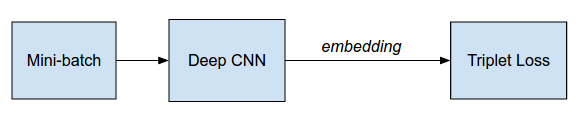
\includegraphics[scale=0.5]{pictures/arch_facenet.png}
\par\large\textit{Figure ?.?: FaceNet architecture.}
\end{center}

\subsection{Triplet Loss} 

Their most significant contribution is so-called "triplet loss". During the training process this loss minimizes the distances between similar faces and maximizes one between different faces.

Loss function that they were using was:
	\begin{align}
	\begin{split}
		 Loss = \sum_{j}^N \left( ||f(x_j^a)-f(x_j^p)||^2_2  - ||f(x_j^a)-f(x_j^n)||^2_2 + \gamma \right)
	\end{split}
	\end{align}
	
where $N$ is a possible set of all triplets in the dataset; $f(x)$ - embedding, that translates image $x$ into Euclidean space; $x_j^a$ - "anchor" image; $x_j^p$ - "positive" image, which should be close to an anchor image; $x_j^n$ - "negative" image; $\gamma$ - margin between positive and negative images.

We are interested in such triplets which violetes the following constraint $||f(x_j^a)-f(x_j^p)||^2_2 + \gamma < ||f(x_j^a)-f(x_j^n)||^2_2$. Only these triplets will contribute to our model during the training process. The only open question how to select such triplets.

They were selecting such pairs where distance between "anchor" and "positive" image was maximized ("hard positive") and the distance between "anchor" and "negative" was as small as possible ("hard negative"), but not zero. It is obviously tricky to look for such triplets in the whole dataset each iteration. Intead they used mini-batch approach to find these "hard positive" and "hard negative" pairs. The size of the batch in their experiments was equal to 1800 examplars.

The problem with selecting hard negatives that $L2$ distance could be equal to 0. Instead they were considering only the cases where the distance of hard positive and anchor less than the distance between hard negative and anchor. They called  them "semi-hard" examplars. 

\subsection{Deep Architectures}

They used two different deep architectures to extract features: 
\begin{itemize}
  \item "Convnet model" developed by D. Zeiler and B. Fergus \cite{zeiler2014visualizing} based on Krizhevsky architecture \cite{krizhevsky2012imagenet}. Model was exteneded by adding $1\times1$ convolutional layer before each standard convolutional layer. These $1\times1$ convolutional kernels were suggested by \cite{min2013nin}. Total number of layers were equal to 22. Number of parameters to train is 140M.
  \item The other model was inspired by "GoogLeNet" Inception convolutional neural network \cite{szegedy2014going}. Their model is almost the same except that they used $L_2$ pooling instead of maxpooling in inception layers. Total number of layers were equal to 16. Number of parameters to train is around 6.6M-7.5M.
\end{itemize}
 
Inception model could be run on the mobile devices because of the small number of parameters to be trained. \par
They used rectified linear units in both these models.

\subsection{Experiments and results}
First I would like to mention that the size of their training dataset is close to 200M faces with 8M identities \cite{schroff2015facenet}, as stated in Table \ref{}. It is the biggest training dataset which exists at this moment in industry. \par
During their experiments they found out that 128 dimension of embedding is good enough for face recognition tasks. It is even possible to use less dimension, 64 for example, without significant loss of accuracy. \par
Both deep architectures showed almost the same results. Except the fact that Inception model is a way better in terms of performance. \par
The most interesting part is how the size of training dataset affects accuracy prediction. They compared the following sizes: millions of images, tens of millions, and hundreds of millions. The most significant impovement was got on the training dataset with tens of millions of examplars. So in their experiments they showed that the question how large your training dataset is important. The larger dataset the more accurate model you will get. But to get all these results they have to run their model for almost 700 hours (~1 month).  \par

Speaking of the accuracy of their model on two academic dataset: LFW and Youtube Faces DB, they achieved current state-of-the-art results. See results in Table ~\ref{tab:table2}.

\begin{table}[!htb]
\centering
\begin{tabular}{|l|l|l|l|l|}
\hline
\multirow{2}{*}{} Models & \multicolumn{2}{l|}{Datasets} \\ \cline{2-3} 
                  &   LFW  &  Youtube Faces DB        \\ \hline
               FaceNet   &  $\textbf{99.63}\% \pm$0.15   &   $\textbf{95.12}\% \pm$0.39       \\ \hline
               DeepFace &  $\textbf{97.35}\% \pm$0.25   &  $\textbf{91.4}\% \pm$1.1       \\ \hline
               Parkhi's approach		& $\textbf{98.65}\%$	 & $\textbf{97.3}\%$ \\ \hline
               DeepID &  $\textbf{97.45}\%$	   &  N/A       \\ \hline
               DeepID2 &  $\textbf{99.15}\%$   &  N/A       \\ \hline
               DeepID2+ &  $\textbf{99.47}\% \pm$0.12   &  $\textbf{93.2}\% \pm$0.2       \\ \hline
               DeepID3 &  $\textbf{99.53}\% \pm$0.1   &  N/A       \\ \hline
               ... & ... & ... \\ \hline
\end{tabular}
\caption{State-of-the-art in face verification.}
\label{tab:table2}
\end{table}

\section{Parkhi's deep face approach}

Inspired by papers \cite{taigman2014deepface, schroff2015facenet}, guys from University of Oxford decided to create their own comparably large face dataset \cite{parkhi2015deep}. And the main reason behind this that these huge datasets from Facebook and Google are not publically available. This newly collected dataset includes 2.6M images belonging to 2,622 unique identities. It is the biggest training dataset for face recognition in the academia at this moment. \par
Besides providing algorithm how to collect this new dataset, they also tested three different models on this dataset from \cite{simonyan2014very}. Using their pretrained model they achieved comparably good results on LFW and YTF to the current state-of-the-art.\par
In terms of face verification problem, they applied the same triplet loss as was suggested here \cite{schroff2015facenet}. For embedding function, was chosen affine projection on Euclidean space.

\subsection{Model architectures}

The architectures A, B and D are same as in \cite{simonyan2014very}. All these three models are same in terms of the type of layers which were used. But they are different in terms of depth. For example, A had 8 convolutional layers and 3 fully-connected (FC) layers. Number of conovlutional layers in B and D models were increased by 2 and 5 respectively. \par 
Input images in all these three models had a size of $224\times224$ pixels. \par
Speaking of the number of filters, they started from 64 and after each max-pooling ($2\times2; stride = 2$) they increased that number twice, until it reached 512. Max-pooling was not applied ater each convolutional layer only at specific places. \par
The main important part of these deep architectures is that very small convolutional kernels ($3\times3$) were used across all convolutional layers. By using these small filters they achieved two goals \cite{simonyan2014very}. First, they reduced the number of parameters that should to be trained. Second improvement they achieved could be extracted from the following fact. 5 by 5 filters, for example, can be represented by the stack of two $3\times3$ consecutive filters without pooling in between. $7\times7$ filters can be replaced by a stack of three $3\times3$ filters. This fact shows us that more disciminative decision function can be learned by replacing one non-linear rectifier units by several ones. \par
The Local Response Normalization (LCN) \cite{krizhevsky2012imagenet} was not used. Because it was shown that LCN does not give any significant improvements in terms of accuracy of their models.

\subsection{Experiments and results}

The evaluation was performed on LFW and YTF datasets, but as the training data they used images from their newly collected dataset. More importantly unique identities from benchmark datasets and new one are different.\par
During the training proces, models B and D used pretrained parameters of A one instead of starting from scratch. \par
They considred several aspects in their experiments on LFW dataset. I will only describe here three of them. First, they evaluated the deep of architectures and how it depends on the accuracy. The experiments showed that B model ($\textbf{97.27}\%$) gave a slight boost in accuracy over model A ($\textbf{96.70}\%$), but model D didn't improve results of model B it performed even worse by giving $\textbf{96.73}\%$ of accuracy. And one of the potential reason for this, that the number of parameters are different. The other one that they used pre-trained parameters from A to train B and D models. By transfering pre-trained parameters one have to be careful with learning rate and momentum. Also they did not investigated random initialization in their experiments. Second, applying 2D allignment on the test dataset gave improvement in accuracy, but applying allignment to training dataset did not improve model. Third, by applying triplet loss they got $\textbf{99.13\%}$ accuracy. It is significant improvements over model B without embedding. \par
To sum it up, they used simpler architecture than was used in DeepID-2,2+,3 \cite{sun2014deep, sun2015deeply, sun2015deepid3} and their model was trained on the smaller dataset comparing to DeepFace and FaceNet approaches. Nevertheless, they achieved comparable results, see Table ~\ref{tab:table2}.


\section{DeepID approach}

\subsection{DeepID}

In this work \cite{sun2014deep} they are considering a problem of classifiying face images to specific person. It is a face identitification problem. The number of unique identities is equal to 10,000. As one can notice, this problem is more challenging comparing to face verification task. They proposed their own deep convolutional network to extract representative features. The architecture of proposed DNN is represented on Fig. ?.?.

\begin{center}
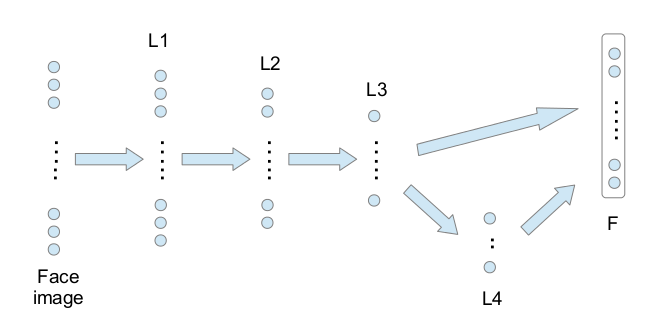
\includegraphics[scale=0.5]{pictures/deepid.png}
\par\large\textit{Figure ?.?: DeepID convolutional network architecture.}
\end{center}

\subsubsection{DeepID architecture}

So their convolutional networks has the following architecture. L1, L2 and L3 represents convolutional layers followed by max-pooling. L4 layer is a last convolutional layer without pooling. F is a vector of learned features. Dimension of the last layer is 160. Moreover, as one can see, the elements of final F layer was formed by projecting features (fully-connected) from L3 and L4 layers. And one of the reasons behind that this type of connection helps to learn multi-scale feature representations \cite{sermanet2011traffic}.  In order to classify face images into one of the specific categories, they added softmax layer, where size was equal to 10,000. F layer and softmax are fully-connected. Rectified linear units (ReLU) was chosen as a non-linear activation function across the whole network. The loss function was a cross-entropy. They used standard Stochastic Gradient descent with backpropagation.

\subsubsection{Face verification problem}

The model from previous section was used to extract features. First, they detected five face points: centers of two eyes, tip of the nose, and two corner points of a mouth. When these fiducial points was detected they applied global similarity transformation. After that they extracted 60 different patches (10 different regions, 3 different scales, and two different color schemes) to train 60 convolutional networks to extract specific features for specific patch. Plus, they considered aligned face image with horizontally flipped image too. So each image was represented by 19,200 ($160\times2\times60$) learned features. \par

In order to solve face verification problem they considered two approaches: Joint Bayesian and neural network. Joint Bayesian approach based on idea of calculating log-likelihood of a pair face images. Proposed neural network for face verification problem had four layers: input layer, two hiddent layers and output one. Input layer represents extracted features from two comparing face images. These features was divided by groups (similar pathes). This input layer was locally connected to the first hidden layer. The purpose of this layer is dimensional reduction and learning similarities between similar patches (local learning). Second hidden layer fully connected with first one. Second layer learns similarities among all these groups (global learning). And the final layer was represented by one unit, which outputs the probability of similarity compared two face images. In order to train this neural network they applied dropout techique to both hidden layers.

\subsubsection{Experiments and results}

DeepID model was trained on CelebA \cite{liu2015faceattributes} dataset and tested on LFW dataset. Both datasets are mutually exclusive. CelebA dataset has 202,599 face images belonging to 10,077 unique identities. $80\%$ of training dataset was used for feature extraction procedure and other $20\%$ for training one of the face verification method. \par

Speaking of the multi-scale approach, combinig both features from third (L3) and forth (L4) layers, to learn final representations (F). Their experiments showed that this type of convolutional network gives almost $5\%$ in error reduction comparing to one without L4 layer. \par

Comparing two methods for face verification problem, Joint Bayesian outperforms neural network by almost $2\%$ on average in accuracy prediction. Their best result on LFW using Joint Bayesian approach gave $97.45\%$ accuracy. It is close to human accuracy on LFW dataset ($97.53\%$).

\subsection{DeepID2}

\begin{center}
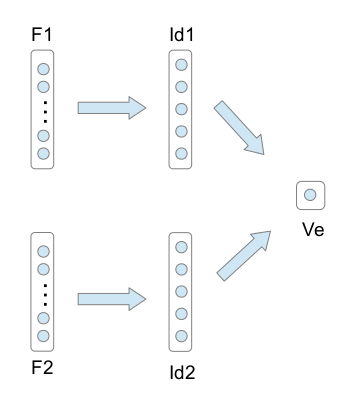
\includegraphics[scale=0.5]{pictures/deepid2.png}
\par\large\textit{Figure ?.?: DeepFace architecture.}
\end{center}

\subsection{DeepID2+}

\begin{center}
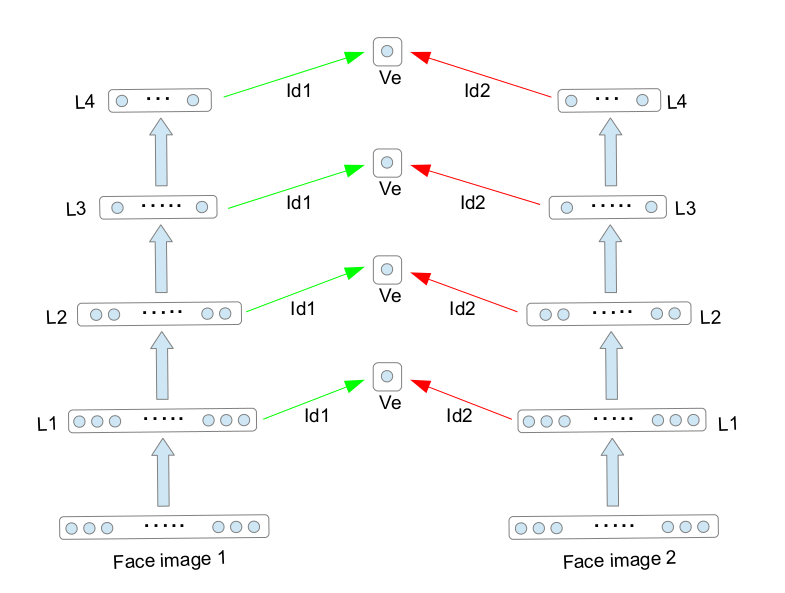
\includegraphics[scale=0.5]{pictures/deepid3.png}
\par\large\textit{Figure ?.?: DeepFace architecture.}
\end{center}

\subsection{DeepID3}

\newpage

\section{Conclusion}
The one drawback of all these large-scale approaches that they didn't use parallelization techniques explained earlier.

\newpage

\bibliographystyle{IEEEtranBST2/IEEEtran}

\bibliography{references}

\end{document}